%%
%% This is file `sample-acmlarge.tex',
%% generated with the docstrip utility.
%%
%% The original source files were:
%%
%% samples.dtx  (with options: `acmlarge')
%% 
%% IMPORTANT NOTICE:
%% 
%% For the copyright see the source file.
%% 
%% Any modified versions of this file must be renamed
%% with new filenames distinct from sample-acmlarge.tex.
%% 
%% For distribution of the original source see the terms
%% for copying and modification in the file samples.dtx.
%% 
%% This generated file may be distributed as long as the
%% original source files, as listed above, are part of the
%% same distribution. (The sources need not necessarily be
%% in the same archive or directory.)
%%
%%
%% Commands for TeXCount
%TC:macro \cite [option:text,text]
%TC:macro \citep [option:text,text]
%TC:macro \citet [option:text,text]
%TC:envir table 0 1
%TC:envir table* 0 1
%TC:envir tabular [ignore] word
%TC:envir displaymath 0 word
%TC:envir math 0 word
%TC:envir comment 0 0
%%
%%
%% The first command in your LaTeX source must be the \documentclass command.
\documentclass[acmlarge]{acmart}
\usepackage{listings}
\lstset{language=Go,
  basicstyle=\ttfamily\scriptsize,
  keywordstyle=\color{blue}\ttfamily,
  stringstyle=\color{red}\ttfamily,
  commentstyle=\color{green}\ttfamily}
%%ss[STYLE]{acmart}
%% \BibTeX command to typeset BibTeX logo in the docs
\AtBeginDocument{%
  \providecommand\BibTeX{{%
    \normalfont B\kern-0.5em{\scshape i\kern-0.25em b}\kern-0.8em\TeX}}}

%% Rights management information.  This information is sent to you
%% when you complete the rights form.  These commands have SAMPLE
%% values in them; it is your responsibility as an author to replace
%% the commands and values with those provided to you when you
%% complete the rights form.
\setcopyright{acmcopyright}
\copyrightyear{2022}
\acmYear{2022}
\acmDOI{}


%%
%% These commands are for a JOURNAL article.
\acmJournal{POMACS}
\acmVolume{37}
\acmNumber{4}
\acmArticle{10}
\acmMonth{8}

%%
%% Submission ID.
%% Use this when submitting an article to a sponsored event. You'll
%% receive a unique submission ID from the organizers
%% of the event, and this ID should be used as the parameter to this command.
%%\acmSubmissionID{123-A56-BU3}

%%
%% The majority of ACM publications use numbered citations and
%% references.  The command \citestyle{authoryear} switches to the
%% "author year" style.
%%
%% If you are preparing content for an event
%% sponsored by ACM SIGGRAPH, you must use the "author year" style of
%% citations and references.
%% Uncommenting
%% the next command will enable that style.
%%\citestyle{acmauthoryear}

%%
%% end of the preamble, start of the body of the document source.
\begin{document}

%%
%% The "title" command has an optional parameter,
%% allowing the author to define a "short title" to be used in page headers.
\title{Paper Presentation of \textit{Chord: A Scalable Peer-to-peer Lookup Service for Internet Applications}}

%%
%% The "author" command and its associated commands are used to define
%% the authors and their affiliations.
%% Of note is the shared affiliation of the first two authors, and the
%% "authornote" and "authornotemark" commands
%% used to denote shared contribution to the research.
\author{Yiwei Yang}
\email{yangyw@shanghaitech.edu.cn}
\orcid{0000-0001-8011-5868}
\affiliation{
  \institution{ShanghaiTech University}
  \streetaddress{1 R.D. Zhongke}
  \city{Shanghai}
  \state{Shanghai}
  \country{China}
  \postcode{21210}
}

%%
%% By default, the full list of authors will be used in the page
%% headers. Often, this list is too long, and will overlap
%% other information printed in the page headers. This command allows
%% the author to define a more concise list
%% of authors' names for this purpose.
\renewcommand{\shortauthors}{Yiwei Yang}

%%
%% The abstract is a short summary of the work to be presented in the
%% article.
\begin{abstract}
  Chord \cite{stoica2003chord}, first proposed by Berkeley Prof. Ion Stoica, is a peer-to-peer distributed hash table mechanism and technique in computing. A distributed hash table maintains key-value pairs by allocating keys to different computers (known as "nodes"); each node will store the values for all of the keys it is responsible for. Chord describes how nodes are assigned keys and how a node can find the value for a particular key by first locating the node accountable for that key.
\end{abstract}

%%
%% The code below is generated by the tool at http://dl.acm.org/ccs.cfm.
%% Please copy and paste the code instead of the example below.
%%
\begin{CCSXML}
  <ccs2012>
  <concept>
  <concept_id>10010520.10010553.10010562</concept_id>
  <concept_desc>Distributed System~Peer to Peer System</concept_desc>
  <concept_significance>500</concept_significance>
  </concept>
  </ccs2012>
\end{CCSXML}

\ccsdesc[500]{Distributed System~Distributed Hash Table}

%%
%% Keywords. The author(s) should pick words that accurately describe
%% the work being presented. Separate the keywords with commas.
\keywords{}


%%
%% This command processes the author and affiliation and title
%% information and builds the first part of the formatted document.
\maketitle
\section{Strong point of the document}

\subsection{The paper introduced another DHT}
Consistent hashing is used to assign a m-bit identification to nodes and keys. For consistent hashing, the SHA-1 algorithm is used as the basis hashing function. Because both keys and nodes (in reality, their IP addresses) are equally distributed in the same identifier space with a small chance of collision, consistent hashing is critical to Chord's robustness and efficiency. As a result, nodes can join and depart the network without causing any interruption. The term node is used in the protocol to refer to both a node and its identification (ID) without ambiguity. The phrase "key" is the same way.

Nodes and keys are arranged in an identifier circle using the Chord lookup protocol, with a maximum of $2^m$ nodes, ranging from 0 to $2^{m-1}-2^m - 1$. ( m should be large enough to avoid colliding with other elements.) Some of these nodes will be associated with machines or keys, while the majority will be vacant.

There is a successor and a predecessor for each node. In a clockwise manner, the successor to a node is the next node in the identifier circle. The predecessor rotates in the other direction. If there is a node for each conceivable ID, node 1 is its successor, and node $2^{m-1}-2^m - 1$ is its predecessor; nevertheless, there are usually "holes" in the sequence.
\subsection{Implementation Detail}

\begin{figure}[htbp]
  \centering
  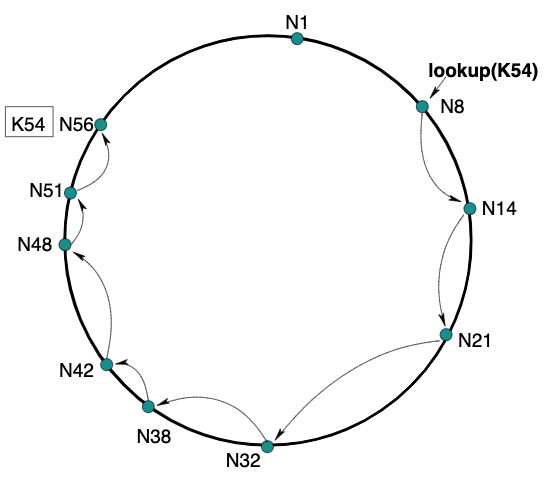
\includegraphics[width=0.4\columnwidth]{./DI.png}
  \caption{Chord Example}
\end{figure}

\subsubsection{Basic query}
The Chord protocol's main purpose is to find successors by querying a key from a client (usually a node) (k). If a node can't discover the key locally, the fundamental technique is to forward the query to the node's successor. The query time will be O(N), where N is the number of machines in the ring.

To avoid the linear search described above, Chord uses a quicker search approach that requires each node to maintain a finger table with up to m entries, where m is the number of bits in the hash key. The $ith$ entry of node n will have the value successor($(n+2^{i-1})\,\bmod\,2^m$). The node's immediate successor is the first element in the finger table (and therefore an extra successor field is not needed). When a node wants to look for a key k, it sends the query to the closest successor or predecessor (depending on the finger table) of k in its finger table (the "biggest" on the circle whose ID is smaller than k) until it discovers the key is stored in its immediate successor.
\subsubsection{Finger table}
In an N-node network, the number of nodes that must be reached to discover a successor using such a finger table is O (log N).
\subsubsection{Node join}
Whenever a new node joins, three invariants should be maintained (the first two ensure correctness and the last one keeps querying fast):
\begin{enumerate}
  \item The successor of each node appropriately points to its immediate successor.
  \item Each key is kept in its own vehicle. successor(k).
  \item The finger table for each node should be correct.
\end{enumerate}
A predecessor field is maintained for each node to meet these invariants. We no longer need to keep this field separate because the successor is the first entry of the finger table. For a newly joined node n, the following tasks should be completed:
\begin{enumerate}
  \item Node n should be initialized (the predecessor and the finger table).
  \item Notify other nodes that their predecessors and finger tables need to be updated.
  \item The new node inherits its successor's responsible keys.
\end{enumerate}
The predecessor of n can readily be found by looking at the predecessor of successor(n) (in the previous circle). There are numerous initialization ways for its finger table. The simplest method is to run find successor queries for all m entries, which will ensure that the $ith$ entry in the finger table is still correct for the $(i+1)th$ entry. This results in O($log2$N). The optimal technique is to update the finger table and initialize it from its immediate neighbors, which is O(log N).

\subsection{Stabilization}

All successor pointers \cite{gummadi2003impact} must be current to ensure correct lookups. As a result, a background stabilization procedure updates finger tables and successor pointers on a regular basis.
\begin{enumerate}
  \item \texttt{Stabilize()}: n requests its predecessor p from its successor and determines whether p should be n's successor instead (this is the case if p recently joined the system).
  \item \texttt{Notify()}: informs n's successor of its existence, allowing it to change n's predecessor.
  \item \texttt{Fix\_fingers()}: updates finger tables
\end{enumerate}
\subsection{The paper have a proof of Complexity and communication cost}
With high probability, can be resolved by contacting O(log N) nodes, where N is the number of nodes in the network.

Suppose node $n$ wishes to find the successor of key $k$. Let $p$ be the predecessor of $k$. We wish to find an upper bound for the number of steps it takes for a message to be routed from $n$ to $p$. Node $n$ will examine its finger table and route the request to the closest predecessor of $k$ that it has. Call this node $f$. If $f$ is the $i^{t h}$ entry in $n$ 's finger table, then both $f$ and $p$ are at distances between $2^{i-1}$ and $2^{2}$ from $n$ along the identifier circle. Hence, the distance between $f$ and $p$ along this circle is at
most $2^{i-1}$. Thus the distance from $f$ to $p$ is less than the distance from $n$ to $f$ : the new distance to $p$ is at most half the initial distance. steps for a message to traverse this remaining distance. The total expected routing time is thus $O(\log N)$.
Simply, the probability that all $r$ nodes fail is $\left(\frac{1}{4}\right)^{r}=O\left(\frac{1}{N}\right)$, which is a low probability; so with high probability at least one of them is alive and the node will have the correct pointer.

\subsection{Chord DHT have many industrial usage}
\begin{enumerate}
  \item Cooperative Mirroring is a load balancing strategy in which a local network hosts information that is accessible to computers on the internet. This approach could allow developers to distribute the load among multiple computers rather than a single server, ensuring that their product is always available.
  \item Distributed Indices: Retrieval of files from a searchable database over the network. P2P file transfer clients, for example.
  \item Time-shared storage: When a computer joins a network, its available data is dispersed throughout the network so that it can be retrieved when the computer disconnects. When a computer is no longer connected to the network, data from other computers is transmitted to the computer in question for offline recovery. Specifically for nodes that are unable to connect to the network on a continuous basis.
  \item Christian Radke: Chord's pessimistic failover strategy whereas in mobile ad hoc networks replicate transmission seems more useful.
\end{enumerate}
\section{Weak point of the document}

We'll not talk about the drawback of DHT here. Despite Chord have advantages like churn rates and low packet loss rate over Pastry \cite{rowstron2001pastry}, it has following drawbacks.
\subsection{Flooding queries}
\begin{figure}[htbp]
  \centering
  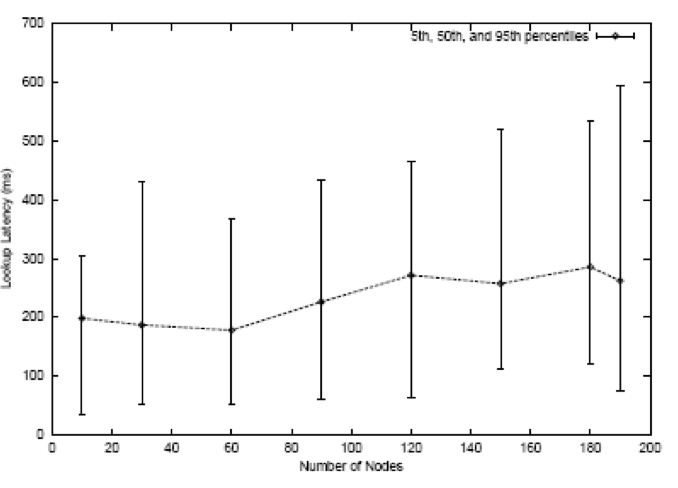
\includegraphics[width=0.3\columnwidth]{./flood.png}
  \caption{Flood Query latency of Chord \cite{lua2005survey}}
\end{figure}

Flooding queries may cause substantial overhead, which means the system's tail latency is pretty high.
\subsubsection{No guarantee of response}
\begin{figure}[htbp]
  \centering
  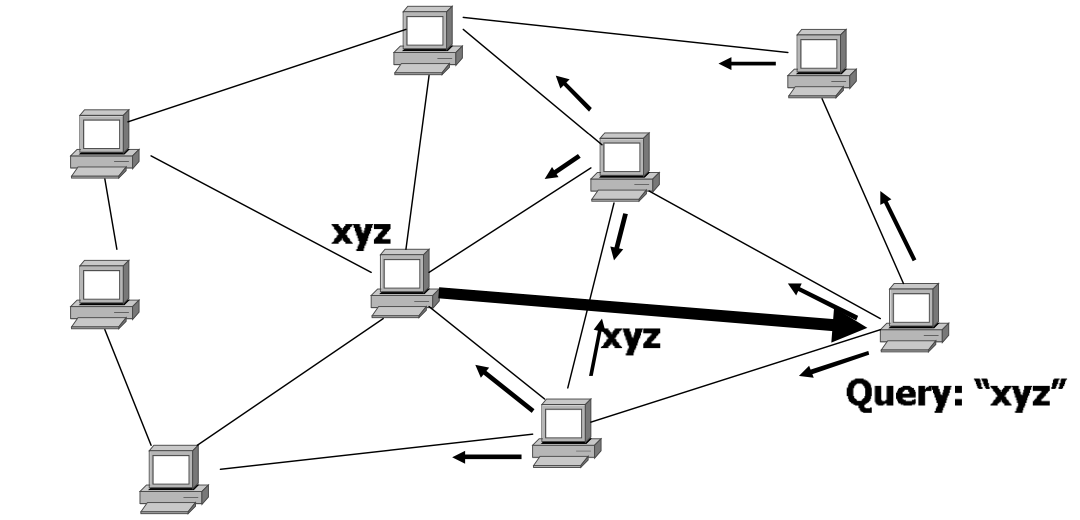
\includegraphics[width=\columnwidth]{./gnutella.png}
  \caption{Overview of Gnutella \cite{cmu}}
\end{figure}

We may not have bounded time for response just like the example in Gnutella.
\begin{enumerate}
  \item Ad-hoc topology
  \item Queries are flooded for bounded number of hops
  \item No guarantees on recall
\end{enumerate}

\subsection{Relatively high route selection}
Here's a comparison of the different DHT system.\\
\begin{tabular}{|c|c|c|c|c|}
  \hline Geometry  & Algorithm & Neighbor Selection                   & Route Selection (log(N) hops)       & Route Selection (> log(N) hops)       \\
  \hline Tree      & Plaxton   & $N^{\log (N) / 2}$                   & 1                                   & 0                                     \\
  \hline Hypercube & CAN       & 1                                    & $c_{1}(\log (\mathrm{N}))$          & 0                                     \\
  \hline Butterfly & Viceroy   & 1                                    & 1                                   & 0                                     \\
  \hline Hybrid    & Tapestry, & $N^{\log (N) / 2}$                   & 1                                   & $c_{2}(\log (\mathrm{N}))$            \\
  \hline Xastry    & Kademila  & $N^{\log (N) / 2}$                   & 1                                   & $\mathrm{c}_{2}(\log (\mathrm{N}))$   \\
  \hline Ring      & Chord     & $\mathrm{N}^{\log (\mathrm{N}) / 2}$ & $\mathrm{c}_{1}(\log (\mathrm{N}))$ & $2 \mathrm{c}_{2}(\log (\mathrm{N}))$ \\
  \hline
\end{tabular}
\section{Possible Refinement to the idea}
\subsection{Minimized the complexity of implementation \texttt{find\_successor}}
The most difficult operation you must support is a complete find successor lookup, which may require numerous servers to be contacted. It should begin by seeing if the result is available locally. If it doesn't, it'll go into a loop. It calls a single server in each iteration and requests the result. The server either returns the result or the forwarding address of the next node to be contacted. 

Just in case, set a hard restriction on the number of requests a single lookup can produce. Create a global, named constant for this. For hundreds of nodes, 32 should suffice.

\begin{lstlisting}
  // ask node n to find the successor of id
  // or a better node to continue the search with
  n.find_successor(id)
      if (id in (n, successor])
          return true, successor;
      else
          return false, closest_preceding_node(id);

  // search the local table for the highest predecessor of id
  n.closest_preceding_node(id)
      // skip this loop if you do not have finger tables implemented yet
      for i = m downto 1
          if (finger[i] in (n,id])
              return finger[i];
      return successor;

  // find the successor of id
  find(id, start)
      found, nextNode = false, start;
      i = 0
      while not found and i < maxSteps
          found, nextNode = nextNode.find_successor(id);
          i += 1
      if found
          return nextNode;
      else
          report error;      
  \end{lstlisting}

\subsection{Memory and Network locality aware notify and find successor}
In Kelips \cite{gupta2003kelips}, real time memory and network time is tested for find nearest locality for find\_successor for better performance.

\bibliographystyle{ACM-Reference-Format}
\bibliography{hoplite_efficient_and_fault_tolerant_collective_communication_for_task_based_distributed_systems}
\end{document}
\endinput
%%
%% End of file `sample-acmlarge.tex'.
